\section{Genetics}\label{sec:genetics}

This section describes important genetic terms that are used throughout the thesis.
They are allele, gene, chromosome, individual, population, crossover, mutation, and reproductive plan.
Also, in subsection~\ref{subsec:schema-theorem}, the Schema Theorem is described, which is an integral part of genetics.

First, it is important to describe what the genetic approach means.
The genetic approach was first introduced by Holland in 1975
to solve optimization problems where it is computationally infeasible to
find an optimal solution by enumerating all possible solutions~\cite{hollandAdaptationNaturalArtificial1975}.

This genetic approach is inspired by nature and Darwin’s Theory of Evolution~\cite{darwinOriginSpeciesMeans2009}
– a population of individuals evolving over time.
Individuals that are more adapted to the environment are
more likely to survive and thus pass their genes to the next generation.
Thus, over time, the population should converge to the state where the adaptation to the environment is the highest.

Holland in~\cite{hollandAdaptationNaturalArtificial1975} defines several structures that reassemble this natural process.
The most important ones are described in the rest of this section.\\

\navesti{Allele} represents a concrete value that a gene can have.
It can be thus described as a set of alternatives to choose from. \\

\navesti{Gene} is a structure composed of alleles.
It often describes one trait or characteristic. \\

\navesti{Chromosome} is a structure composed of genes.
Thus it is an amalgam of characteristics described by genes.\\

\navesti{Individual} is defined by its chromosome and represents a solution to the problem or a structure from which a solution can be constructed.
A numeric value called \textit{fitness} can be assigned to each individual that represents how well the individual performs in an environment. \\

\navesti{Population} is a set of individuals.
It can be interpreted as a subset of possible solutions.\\

One concrete example of the definitions mentioned above is in figure~\ref{fig:population}.
There are two individuals in the population, with their chromosomes having two genes.
The first gene is a vector with alleles having values 1 to 5. The second gene is a string vector
with alleles having values $H$ or $V$. Lastly, each individual has a fitness value.
Thus, because A’s fitness $30.5$ is greater than B’s fitness $9.8$, we can say
that individual A performs better than B.


\begin{figure}
    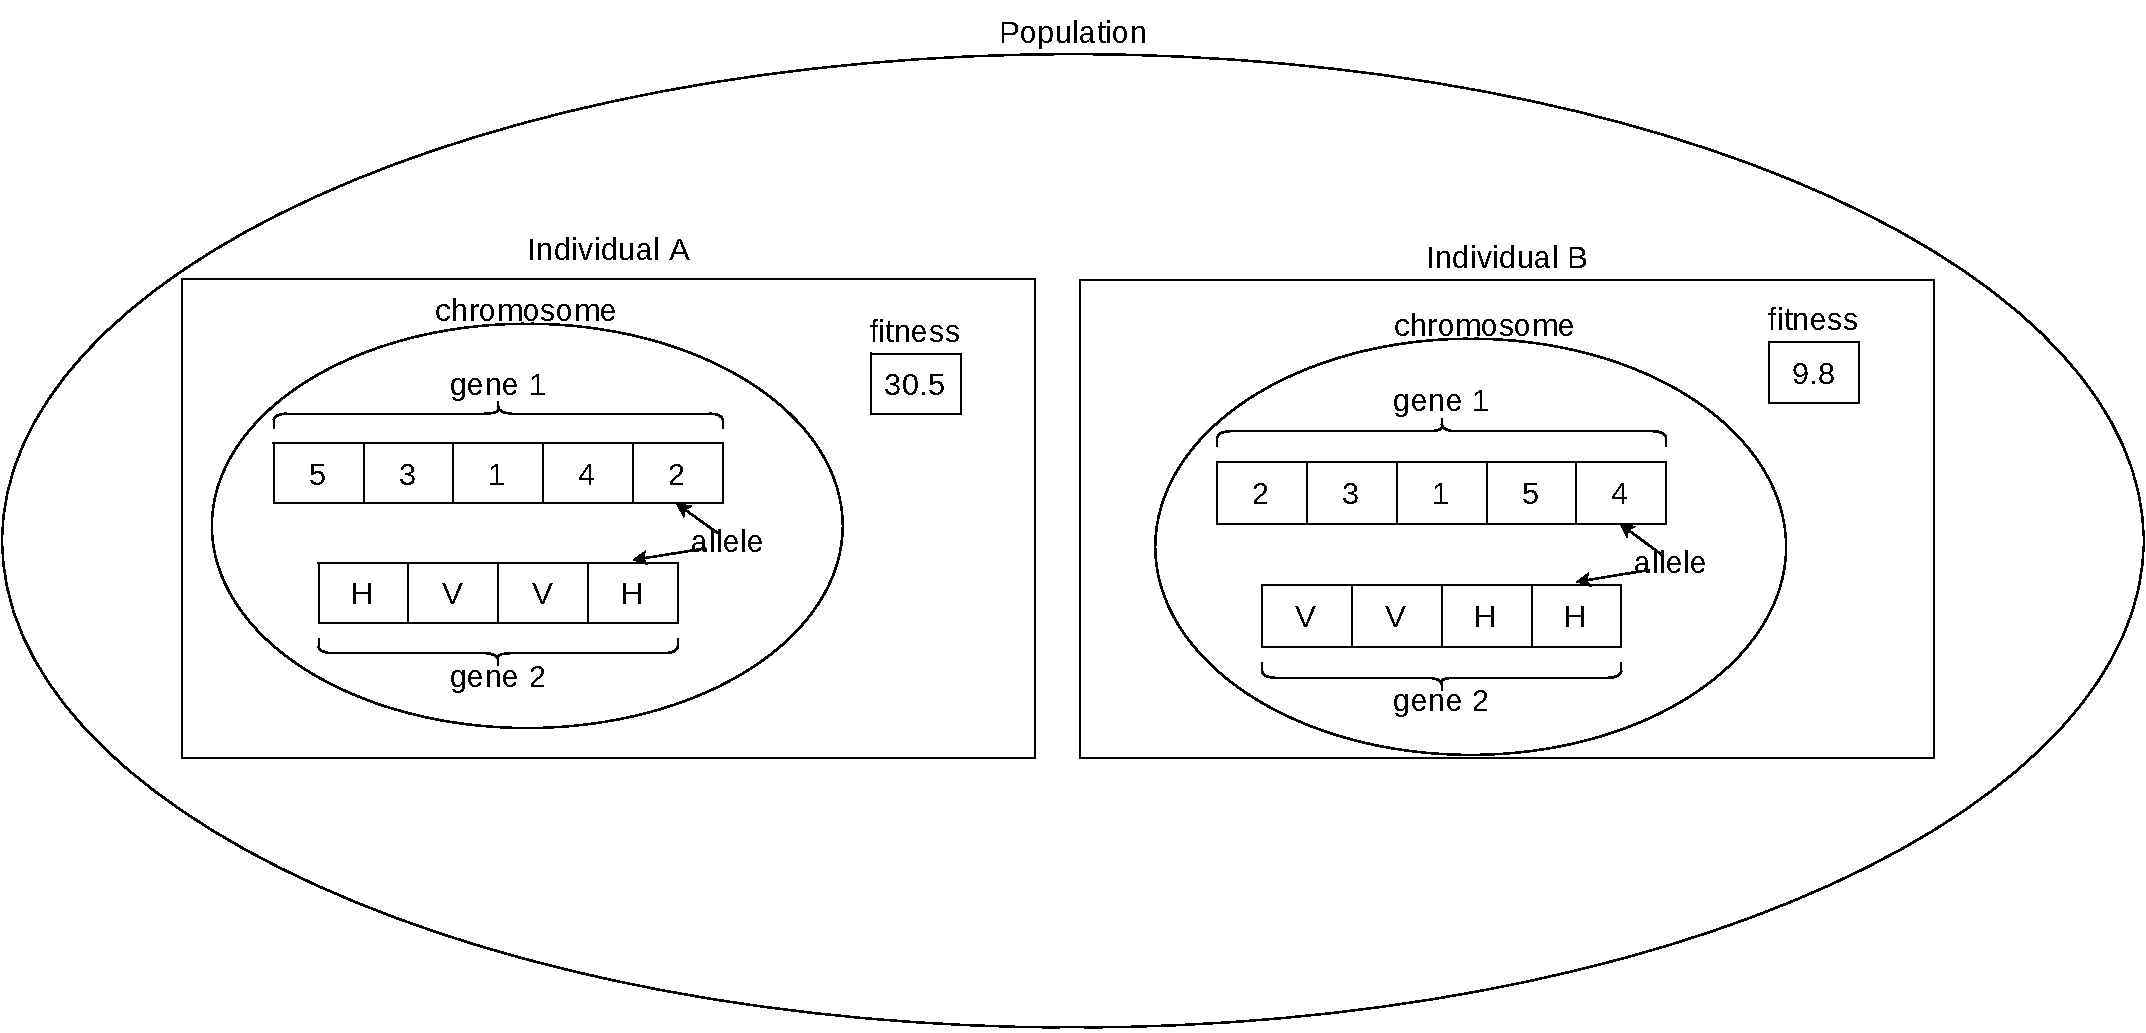
\includegraphics[width=1\textwidth, left]{population}
    \caption[Population example]{Example of a population composed of two individuals.}
    \label{fig:population}
\end{figure}

For the structures defined above, multiple operations called \textit{genetic operators}
are defined by Holland and used by other researchers following his work.
Genetic operators aim to create new individual/s using individuals already present in a population as input.
Two of them that are used in this thesis are described below.\\


\navesti{Crossover} genetic operator takes two individuals as input and, by recombination
of their alleles in their genes, produces a new individual/s called \textit{offspring} or \textit{child}.\\

\navesti{Mutation} genetic operator takes one individual as input and produces a new one
which may have some of its alleles replaced by different ones at random.\\

Finally, there needs to be a process that transforms a population
to a new one with the goal of if this transformation process is applied sufficient
number of times to some initial population,
(sub)-optimal solution to the problem will be found.
This process is called \textit{reproductive plan}.\\

\navesti{Reproductive plan} is a process that takes a population on input and produces a modified
population using genetic operators.\\

One example of a reproductive plan is in figure~\ref{fig:reproductive-plan}.
At the start, an initial population of individuals is generated.
Then, for each individual, the fitness value is calculated.
Lastly, two genetic operators are applied to produce the new population.
In this example, crossover and mutation.
The process ends if the stopping condition is met.

\begin{figure}[h]
    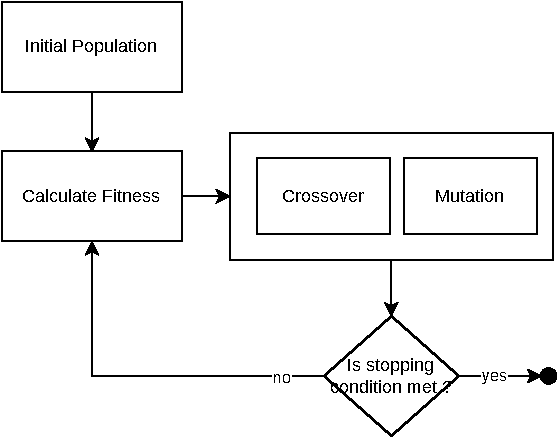
\includegraphics[width=0.65\textheight, center]{reproductive_plan}
    \caption[Example of a reproductive plan]{Example of a reproductive plan with crossover and mutation genetic operators.}
    \label{fig:reproductive-plan}
\end{figure}

\subsection{Schema Theorem}\label{subsec:schema-theorem}

Holland in~\cite{hollandAdaptationNaturalArtificial1975} proposed
the Schema Theorem arguing why the genetic approach described above works.
This subsection describes the main idea behind the argument.

First, let us say that a \textit{schema} is an extended representation of chromosome,
where each gene can contain a “don’t care” symbol marked as underscore $\_$.
This symbol can take up any value that an allele can in the given context.
We can then say that chromosome belongs to a schema
and that schema contains a chromosome.

Schema can be illustrated on chromosomes with one gene represented as
a vector that contains a permutation of numbers $1$ to $7$.
Then, example of a schema is $H_1 = \langle 5, \_, \_, 2, \_, 3, \_ \rangle$.
It contains $24$ chromosomes, with one example being $\langle 5, 4, 1, 2, 6, 3, 7 \rangle$.
On the other hand, schema $H_2 = \langle 1, 2, 3, 4, 5, 6, \_ \rangle$ contains only one chromosome.

There are other properties that a schema has – length and order.
\textit{Length} is the distance from the first “non-don’t care” symbol to the last.
\textit{Order} is the number of “non-don’t care” symbols contained in the schema.
For example, $H_1$ has length $6$ and order $3$.
It is graphically illustrated in figure~\ref{fig:schema}.
On the other hand, schema $H_2$ has the same length, $6$, but higher order, which is also $6$.

With schema being defined, we can interpret any population of individuals as a pool of schemata.
It can then be reformulated that a genetic approach, which has a reproductive plan and
genetic operators, (1) creates new schemata by recombination of the one already present in the population,
(2) creates schemata that are not present in the population, and (3) keeps a history of the best schemata found.
The Schema Theorem can then be written as

\begin{equation}
    \mathrm{E}[M(H, t+1)] \geq M(H, t) \dfrac{\mu(H)}{\overline{\mu}}\left[ 1 - p_c \dfrac{\delta(H)}{k-1} - \sigma(H)
    p_m \right]\,,
    \label{eq:schema-theorem}
\end{equation}

where $M(H, t)$ is expected number of individuals whose chromosome belongs to schema $H$ in population $t$,
$\mu(H)$ is average fitness of individuals whose chromosome belongs to $H$,
$\overline{\mu}$ is average population fitness,
$\delta(H)$ is length of schema $H$ with it’s maximum length $k$,
$\sigma(H)$ is order of $H$,
$p_c$ is crossover probability, and
$p_m \ll 1$ is mutation probability.

Inequality~\ref{eq:schema-theorem} says, that the success of a schema $H$,
considering only crossover and low probability mutation are purely determined
by its better-than-average performance, length, and order.
It can be thus reformulated that the genetic approach favors
short schemata with low order that have better-than-average performance.

The reasoning behind the argument is that schemata with high order are more likely
to be damaged by mutation, i.e., an allele of a schema is replaced by a different one.
Also, longer schemata are more likely to be split using a crossover, whereas Holland
considers a one-point-crossover that produces an offspring’s chromosome by copying
first half of the first parent’s chromosome followed by the second’s parent second half of the chromosome.

\begin{figure}[h]
    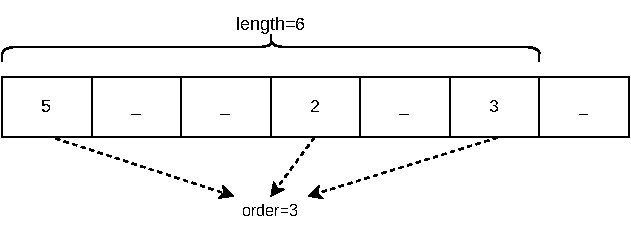
\includegraphics[width=0.7\textwidth, center]{schema}
    \caption[Example of a schema]{Example of a schema, where “don’t care” symbol marked as underscore $\_$.}
    \label{fig:schema}
\end{figure}
